\documentclass[10pt]{beamer}
\usetheme[progressbar=frametitle]{metropolis}
\usepackage{tikz}
\usetikzlibrary{positioning,arrows,shapes,fit,calc}
\usepackage{appendixnumberbeamer}
\usepackage[svgnames,table]{xcolor}
\usepackage{tabularx}
\usepackage{booktabs}
\usepackage[scale=2]{ccicons}
\usepackage{adjustbox}
\usepackage{pifont}
\usepackage{pgfplots}
\usepgfplotslibrary{dateplot}
\usepackage{xspace}
\usepackage{amsmath,amssymb}

\newcommand{\themename}{\textsc{metropolis}\xspace}

% Math commands
\newcommand{\E}{\mathbb{E}}
\renewcommand{\max}{\text{max}}
\renewcommand{\min}{\text{min}}
\newcommand{\argmax}{\text{argmax}}

\title{Dynamic Programming and Reinforcement Learning}
\date{April 2025}
\author{Pranjal Rawat}
\institute{Georgetown University}

\begin{document}

\maketitle

%==============================================================
% SECTION 1: INTRODUCTION AND FOUNDATIONS
%==============================================================

\section{Introduction and Foundations}

%----------------------------------
% Introduction & Motivation
%----------------------------------

\begin{frame}{Introduction \& Motivation}
    \begin{itemize}
        \item Many economic decisions are inherently dynamic and strategic: 
        \begin{itemize}
            \item Investment timing (Dixit \& Pindyck, 1994)
            \item Optimal stopping (McCall, 1970)
            \item Market entry/exit (Ericson \& Pakes, 1995)
        \end{itemize}
        \vspace{0.2cm}
        \item Traditional approaches in economics:
        \begin{itemize}
            \item Analytical solutions (simplified models)
            \item Numerical dynamic programming (limited dimensions)
        \end{itemize}
        \vspace{0.2cm}
        \item Computational challenges:
        \begin{itemize}
            \item Identification
            \item Curse of dimensionality
            \item Multiplicity of Equilibria
        \end{itemize}
    \end{itemize}
\end{frame}

\begin{frame}{Introduction \& Motivation (cont.)}
    \begin{itemize}
        \item Questions we'll address:
        \begin{itemize}
            \item How can we efficiently solve complex decision problems?
            \item What are the trade-offs between different solution methods?
            \item How can reinforcement learning complement traditional approaches?
            \item What are potential applications to economic modeling?
        \end{itemize}
    \end{itemize}
\end{frame}

%----------------------------------
% MDPs and Policies
%----------------------------------

\begin{frame}{MDPs and Policies}
    \begin{itemize}
        \item MDP defined as tuple $(S, A, P, R, \gamma)$:
        \begin{itemize}
            \item $S$: State space (e.g., inventory levels, market conditions)
            \item $A$: Action space (e.g., investment, pricing, production)
            \item $P(s'|s,a)$: Transition probability
            \item $R(s,a,s')$: Reward function (e.g., profits, utility)
            \item $\gamma \in [0,1)$: Discount factor (time preference)
        \end{itemize}
        \vspace{0.2cm}
        \item Policy $\pi$: Mapping from states to actions
        \begin{itemize}
            \item Deterministic: $\pi(s) \in A$
            \item Stochastic: $\pi(a|s)$ as probability distribution
        \end{itemize}
    \end{itemize}
\end{frame}

%----------------------------------
% Value Functions
%----------------------------------

\begin{frame}{Value Functions}
    \begin{itemize}
        \item State-value function for policy $\pi$:
        \begin{equation}
            V^{\pi}(s) = \E_{\pi}\left[\sum_{t=0}^{\infty} \gamma^t R(s_t, a_t, s_{t+1}) \,\middle|\, s_0 = s\right]
        \end{equation}
        
        \item Action-value function for policy $\pi$:
        \begin{equation}
            Q^{\pi}(s,a) = \E_{\pi}\left[\sum_{t=0}^{\infty} \gamma^t R(s_t, a_t, s_{t+1}) \,\middle|\, s_0 = s, a_0 = a\right]
        \end{equation}
        
        \item Economic interpretation:
        \begin{itemize}
            \item $V^{\pi}(s)$: Expected present value of future rewards under policy $\pi$
            \item $Q^{\pi}(s,a)$: Expected present value when taking action $a$ then following $\pi$
        \end{itemize}
    \end{itemize}
\end{frame}

\begin{frame}{Optimal Value Functions and Policy}
    \begin{itemize}
        \item Optimal value functions:
        \begin{align}
            V^*(s) &= \max_{\pi} V^{\pi}(s) \\
            Q^*(s,a) &= \max_{\pi} Q^{\pi}(s,a)
        \end{align}
        
        \item Bellman optimality equations:
        \begin{align}
            V^*(s) &= \max_a \sum_{s'} P(s'|s,a) \left[ R(s,a,s') + \gamma V^*(s') \right]
        \end{align}
        
        \item Optimal policy:
        \begin{equation}
            \pi^*(s) = \argmax_a Q^*(s,a)
        \end{equation}
        
        \item Economic interpretation: $V^*(s)$ is the maximum attainable present value from state $s$
    \end{itemize}
\end{frame}

%----------------------------------
% Asset Replacement Example
%----------------------------------

\begin{frame}{Asset Replacement}
    \begin{itemize}
        \item Economic maintenance problem:
        \begin{itemize}
            \item States: Asset quality $s \in \{1,2,3\}$ (good, fair, poor)
            \item Actions: Replace (R) or Keep (K)
            \item Rewards:
            \begin{itemize}
                \item $R(s,\text{K}) = 4-s$ (higher quality → higher rewards)
                \item $R(s,\text{R}) = 1-s$ (replacement cost increases with deterioration)
            \end{itemize}
            \item Transitions:
            \begin{itemize}
                \item Replace: $P(s'=1|s,\text{R})=1$ for all $s$ (reset to good quality)
                \item Keep: Asset deteriorates stochastically
            \end{itemize}
            \item Discount factor: $\gamma = 0.9$
        \end{itemize}
    \end{itemize}
\end{frame}

\begin{frame}{Asset Replacement}
\begin{center}
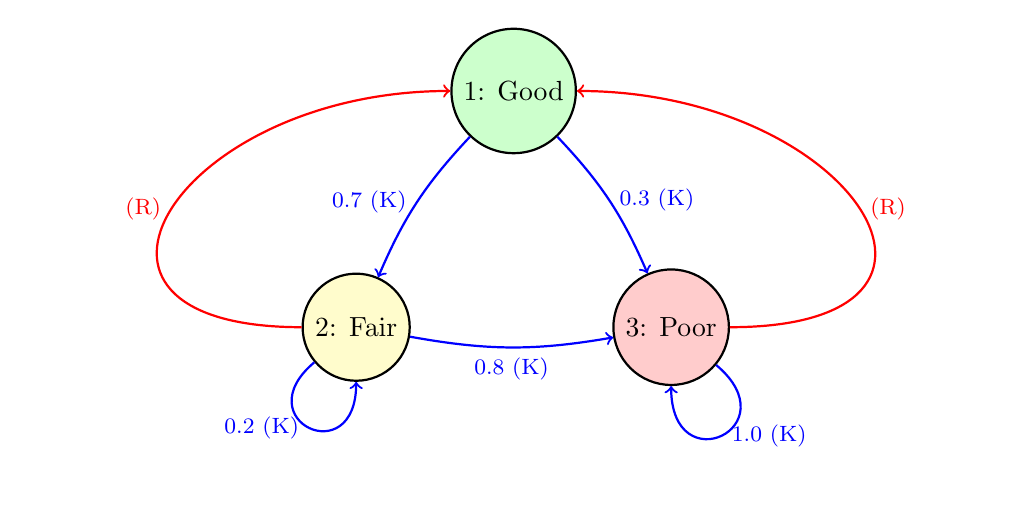
\begin{tikzpicture}[
    scale=1.0,
    node/.style={circle, draw, thick, minimum size=1.3cm, font=\normalsize},
    label/.style={font=\footnotesize}
]
    % Triangle arrangement
    \node[node, fill=green!20] (S1) at (0,2)   {$1$: Good};
    \node[node, fill=yellow!20] (S2) at (-2,-1)  {$2$: Fair};
    \node[node, fill=red!20] (S3) at (2,-1) {$3$: Poor};
    
    % Keep transitions (blue)
    \draw[->, thick, blue] (S1) to[bend right=10] 
        node[label, left] {$0.7$ (K)} (S2);
    \draw[->, thick, blue] (S2) to[bend right=10] 
        node[label, below] {$0.8$ (K)} (S3);
    \draw[->, thick, blue] (S1) to[bend left=10] 
        node[label, right] {$0.3$ (K)} (S3);
        
    % Self loops
    \draw[->, thick, blue] (S2) to[out=220, in=270, looseness=5] 
        node[label, left] {$0.2$ (K)} (S2);
    \draw[->, thick, blue] (S3) to[out=320, in=270, looseness=5] 
        node[label, right] {$1.0$ (K)} (S3);
    
    % Replace transitions (red) - MORE LOOPY with wider spread
    \draw[->, thick, red] (S2) to[out=180, in=180, looseness=2.5] 
        node[label, left] {(R)} (S1);
    \draw[->, thick, red] (S3) to[out=0, in=0, looseness=2.5] 
        node[label, right] {(R)} (S1);
\end{tikzpicture}
\end{center}

\begin{itemize}
    \item Optimal policy: keep if $s=1$ or $s=2$; replace if $s=3$.
    \item Intuition: replace only when the asset is in poor condition.
\end{itemize}
\end{frame}

%==============================================================
% SECTION 2: SOLUTION METHODS
%==============================================================

\section{Solution Methods}

%----------------------------------
% Value Iteration
%----------------------------------

\begin{frame}{Value Iteration (DP)}
    \begin{itemize}
        \item Iteratively applies Bellman optimality operator:
        \begin{equation}
            \hat{V}_{k+1}(s) = \max_a \sum_{s'} P(s'|s,a) \left[ R(s,a,s') + \gamma \hat{V}_k(s') \right]
        \end{equation}
        
        \item Algorithm:
        \begin{enumerate}
            \item Initialize $\hat{V}_0(s) = 0$ for all $s \in S$
            \item Repeat until convergence:
            \begin{itemize}
                \item For each state $s$, compute $\hat{V}_{k+1}(s)$ using the equation above
                \item Check if $\max_s |\hat{V}_{k+1}(s) - \hat{V}_k(s)| < \epsilon$
            \end{itemize}
            \item Extract policy: $\hat{\pi}(s) = \argmax_a \sum_{s'} P(s'|s,a) [R(s,a,s') + \gamma \hat{V}(s')]$
        \end{enumerate}
    \end{itemize}
\end{frame}

\begin{frame}{Value Iteration: Properties}
    \begin{itemize}
        \item Key properties:
        \begin{itemize}
            \item Model-based: Requires explicit transition and reward model
            \item Guaranteed convergence: $\hat{V}_k \to V^*$ at rate $\gamma$
        \end{itemize}
        \vspace{0.2cm}
        \item Economic applications:
        \begin{itemize}
            \item Optimal growth models (Stokey \& Lucas, 1989)
            \item Asset pricing with discrete states 
            \item Discrete choice dynamic programming (Rust, 1994)
        \end{itemize}
        \vspace{0.2cm}
        \item Limitations:
        \begin{itemize}
            \item State space grows exponentially
            \item Requires full model specification
        \end{itemize}
    \end{itemize}
\end{frame}

%----------------------------------
% Policy Iteration
%----------------------------------

\begin{frame}{Policy Iteration (DP)}
    \begin{itemize}
        \item Alternates between two phases:
        
        \item 1. Policy evaluation: Compute value of current policy $\hat{\pi}_k$
        \begin{equation}
            \hat{V}^{\hat{\pi}_k}(s) = \sum_{s'} P(s'|s,\hat{\pi}_k(s)) \left[ R(s,\hat{\pi}_k(s),s') + \gamma \hat{V}^{\hat{\pi}_k}(s') \right]
        \end{equation}
        
        \item 2. Policy improvement: Find better policy $\hat{\pi}_{k+1}$
        \begin{equation}
            \hat{\pi}_{k+1}(s) = \argmax_a \sum_{s'} P(s'|s,a) \left[ R(s,a,s') + \gamma \hat{V}^{\hat{\pi}_k}(s') \right]
        \end{equation}
        
        \item Compared to value iteration:
        \begin{itemize}
            \item Typically fewer iterations until convergence
            \item More computation per iteration (solving linear system)
        \end{itemize}
    \end{itemize}
\end{frame}

%----------------------------------
% Generalized Policy Iteration
%----------------------------------

\begin{frame}{Generalized Policy Iteration}
    
    \begin{itemize}
        \item All solution methods follow this pattern:
        \begin{itemize}
            \item Evaluate or estimate the value of current policy
            \item Improve policy based on value estimates
        \end{itemize}
        \item Differences:
        \begin{itemize}
            \item How much evaluation before improvement
            \item How the evaluation is performed (model vs. samples)
            \item How improvement is performed
        \end{itemize}
    \end{itemize}
\end{frame}

%----------------------------------
% Q-Learning
%----------------------------------

\begin{frame}{Q-Learning (RL)}
    \begin{itemize}
        \item Model-free temporal difference learning:
        \begin{equation}
            \hat{Q}(s,a) \leftarrow \hat{Q}(s,a) + \alpha \left[ R + \gamma \max_{a'} \hat{Q}(s',a') - \hat{Q}(s,a) \right]
        \end{equation}
        
        \item Algorithm:
        \begin{enumerate}
            \item Initialize $\hat{Q}(s,a) = 0$ for all $s \in S, a \in A$
            \item Repeat for each episode:
            \begin{itemize}
                \item Initialize state $s$
                \item For each step in episode:
                \begin{itemize}
                    \item Choose action $a$ from $s$ using policy derived from $\hat{Q}$ (e.g., $\epsilon$-greedy)
                    \item Take action $a$, observe reward $R$ and next state $s'$
                    \item Update $\hat{Q}(s,a)$ using the equation above
                    \item $s \leftarrow s'$
                \end{itemize}
            \end{itemize}
        \end{enumerate}
    \end{itemize}
\end{frame}

\begin{frame}{Q-Learning: Properties}
    \begin{itemize}
        \item Key characteristics:
        \begin{itemize}
            \item No model required (learns from experience)
            \item Off-policy: Updates using max operator regardless of actual next action
            \item Bootstrapping: Uses current estimates for future values
            \item Exploration-exploitation trade-off (typically $\epsilon$-greedy)
        \end{itemize}
        \vspace{0.2cm}
        \item Convergence guarantees:
        \begin{itemize}
            \item $\hat{Q} \to Q^*$ with probability 1 under appropriate conditions
            \item Requires sufficient exploration and proper learning rate schedule
        \end{itemize}
        \vspace{0.2cm}
    \end{itemize}
\end{frame}

%----------------------------------
% Monte Carlo Control
%----------------------------------

\begin{frame}{Monte Carlo Control (RL)}
    \begin{itemize}
        \item Episode-based learning from complete returns:
        \begin{equation}
            \hat{Q}(s_t,a_t) \leftarrow \hat{Q}(s_t,a_t) + \alpha \left[ G_t - \hat{Q}(s_t,a_t) \right]
        \end{equation}
        where $G_t = \sum_{k=0}^{T-t-1} \gamma^k R_{t+k+1}$ is the actual return
        
        \item Key characteristics:
        \begin{itemize}
            \item No bootstrapping: Uses actual outcomes (unbiased estimates)
            \item No model required (learns from experience)
            \item Requires episodic tasks with well-defined termination
            \item High variance, no bias
        \end{itemize}
        
        \item Economic applications:
        \begin{itemize}
            \item Option pricing (Longstaff \& Schwartz, 2001)
            \item Market entry with finite horizons
        \end{itemize}
    \end{itemize}
\end{frame}

\begin{frame}{Width vs Depth}
Dynamic programming is width-first while Monte Carlo methods are depth-first. 
\begin{figure}
    \centering
    
\includegraphics[width=0.7\linewidth]{figs/map.jpg}
    %\caption{Caption}
    \label{fig:enter-label}
\end{figure}
\end{frame}

%----------------------------------
% REINFORCE - Policy Gradient
%----------------------------------

\begin{frame}{Policy Gradient Methods}

    \begin{itemize}
        \item Directly optimize parameterized policy $\pi_\theta(a|s)$
        \item Objective function (expected return):
        \begin{equation}
            J(\theta) = \E_{\tau \sim \pi_\theta} \left[ \sum_{t=0}^{T} \gamma^t r_t \right]
        \end{equation}
        where $\tau$ is a trajectory $(s_0, a_0, r_1, s_1, \ldots)$
        
        \item Policy gradient update (REINFORCE):
        \begin{equation}
            \theta \leftarrow \theta + \alpha \nabla_\theta \hat{J}(\theta)
        \end{equation}
        
    \end{itemize}
\end{frame}

%----------------------------------
% Planning vs Learning
%----------------------------------

\begin{frame}{Unified View: Planning vs. Learning}
    \begin{columns}
        \begin{column}{0.5\textwidth}
            \textbf{Planning}
            \begin{itemize}
                \item Uses a model to imagine the future
                \item Requires complete model:
                \begin{itemize}
                    \item $P(s'|s,a)$ known
                    \item $R(s,a,s')$ known
                \end{itemize}
                \item Can evaluate many actions before taking any
                \item Examples: Value Iteration, Policy Iteration
            \end{itemize}
        \end{column}
        
        \begin{column}{0.5\textwidth}
            \textbf{Learning}
            \begin{itemize}
                \item Actually takes steps in environment
                \item Model-free:
                \begin{itemize}
                    \item Only needs samples $(s,a,r,s')$
                    \item No explicit knowledge of dynamics
                \end{itemize}
                \item Must balance exploration/exploitation
                \item Examples: Q-Learning, Monte Carlo, REINFORCE
            \end{itemize}
        \end{column}
    \end{columns}
\end{frame}

%==============================================================
% SECTION 3: APPLICATIONS
%==============================================================

\section{Applications}

%----------------------------------
% Grid World - Description
%----------------------------------

\begin{frame}{Grid World: Setup}
    \begin{itemize}
        \item 5$\times$5 grid, states are positions $(row,col)$
        \item Actions: Left, Right, Up, Down, Stay
        \item Transitions: Deterministic, bounded by grid edges
        \item Rewards:
        \begin{itemize}
            \item +10 at goal (4,4)
            \item Small state rewards, $-0.1$ movement cost
        \end{itemize}
        \item Discount factor: $\gamma = 0.95$
        \item Example: Taxi Routing
\end{itemize}
\end{frame}


\begin{frame}{Grid World Navigation: Paths Found}
    \begin{columns}
        \begin{column}{1.0\textwidth}
            \begin{figure}
                
\includegraphics[width=\textwidth]{figs/paths.png}
                %\caption{Grid world with goal at (4,4)}
            \end{figure}
        \end{column}
    \end{columns}
\end{frame}

%----------------------------------
% Deep Q-Networks
%----------------------------------

\begin{frame}{Deep Q-Networks (DQN)}
    \begin{itemize}
        \item Function approximation:
        \begin{equation}
            Q(s,a;\theta) \approx Q^*(s,a)
        \end{equation}
        $\theta$ are the neural network weights.

        \item Loss function:
        \begin{equation}
            \mathcal{L}(\theta) = \mathbb{E}_{(s,a,r,s') \sim \mathcal{D}} \left[ \left( y - Q(s,a;\theta) \right)^2 \right]
        \end{equation}
        where target $y = r + \gamma \max_{a'} Q(s', a'; \theta^-)$ and $\theta^-$ is the target network.

        \item Stabilization techniques:
        \begin{itemize}
            \item Experience replay: buffer $\mathcal{D}$ stores past transitions to decorrelate updates
            \item Target network: $\theta^-$ is a lagged copy of $\theta$, updated periodically
        \end{itemize}
    \end{itemize}
\end{frame}


%----------------------------------
% Capital Replacement - Problem
%----------------------------------

\begin{frame}{Capital Replacement Problem}
    \begin{itemize}
        \item Economic maintenance optimization problem:
        \begin{itemize}
            \item $N$ parallel engines with mileage states $m_i \in \{0,1,2,3,4,5\}$
            \item System state $s = (m_1,...,m_N)$
            \item Action space $A(s)$: All subsets of engines to replace
            \item Capacity constraint: Maximum 3 engines can be replaced at once
        \end{itemize}
        \vspace{0.2cm}
        \item Cost function:
        \begin{equation}
            c(s,a) = \alpha \sum_{i=1}^{N} \mathbf{1}_{m_i > 0} + \beta |a|
        \end{equation}
        where:
        \begin{itemize}
            \item $\alpha=1.0$ is the cost of aged engines
            \item $\beta=5.0$ is the replacement cost per engine
            \item $|a|$ is the number of replaced engines
        \end{itemize}
        \vspace{0.2cm}
        \item State transitions: Engines are reset to state 0 when replaced, otherwise age by 1
    \end{itemize}
\end{frame}

%----------------------------------
% Capital Replacement - Results
%----------------------------------

\begin{frame}{Capital Replacement Results: DP vs DQN}
    \begin{table}
        \centering
        \small
        \begin{tabular}{cccccc}
            \toprule
            $N$ & \#States & DP Time (s) & DP Reward & DQN Time (s) & DQN Reward \\
            \midrule
            3 & 216 & 0.29 & -59.42 & 6.27 & -59.53 \\
            4 & 1,296 & 3.64 & -79.35 & 23.60 & -79.43 \\
            5 & 7,776 & 44.82 & -99.26 & 111.33 & -99.15 \\
            6 & 46,656 & 500.98 & -119.10 & 67.81 & -118.88 \\
            7 & 279,936 & $\sim$6418.84 & -- & 64.18 & -138.93 \\
            \bottomrule
        \end{tabular}
    \end{table}
    
    \begin{itemize}
        \item Key findings:
        \begin{itemize}
            \item Small instances ($N \leq 3$): DP provides exact solutions rapidly
            \item Medium instances ($4 \leq N \leq 6$): Both viable, but DP time grows exponentially
            \item Large instances ($N \geq 7$): DP becomes intractable, DQN remains efficient
        \end{itemize}
        \item DQN reward error typically $< 1\%$ compared to exact DP solution
    \end{itemize}
\end{frame}

%----------------------------------
% RL in Operations Research
%----------------------------------

\begin{frame}{RL Applications in Operations Research}
    \begin{itemize}
        \item Inventory management:
        \begin{itemize}
            \item Boute et al. (2022): Deep RL matches specialized heuristics in complex inventory problems
            \item 30-40\% cost reduction vs. standard policies in multi-item settings
        \end{itemize}
        \vspace{0.2cm}
        \item Maintenance optimization:
        \begin{itemize}
            \item Sabri et al. (2024): Attention-based DRL delivers 30.5\% lower costs than DP-based heuristics for combinatorial maintenance scheduling
            \item Seconds vs. hours computation time
        \end{itemize}
        \vspace{0.2cm}
        \item Dynamic pricing:
        \begin{itemize}
            \item Nomura et al. (2025): PPO achieved near-optimal solutions with 75\% reduction in computation time compared to DP for perishable inventory with dynamic pricing
        \end{itemize}
    \end{itemize}
\end{frame}

%----------------------------------
% Soft Actor-Critic
%----------------------------------

\begin{frame}{MDPs for Robot Learning: Quadruped Walking}
    \begin{itemize}
        \item Context:
        \begin{itemize}
            \item Learning to walk requires coordinated motor control
            \item Traditional RL methods require extensive real-world interaction
            \item Model-based approach enables sample-efficient learning
            \item Quadruped learns to roll, stand, and walk from scratch
        \end{itemize}
        \vspace{0.2cm}
        \item MDP formulation:
        \begin{itemize}
            \item States $S$: Joint angles, velocities, body orientation, contact forces
            \item Actions $A$: Torque controls for 8 joints (hip, knee for each leg)
            \item Transition $P(s'|s,a)$: Complex leg-ground interactions and physics
            \item Rewards $R(s,a)$: Forward velocity, energy efficiency, stability
            \item $\gamma$: Discount factor balancing immediate vs. future stability
        \end{itemize}
        \vspace{0.2cm}
        \item Training process (Dreamer):
        \begin{itemize}
            \item World model learns environment dynamics from experience
            \item Planning performed in imagination to reduce physical interaction
            \item Achieves walking in 1 hour without simulation or manual resets
        \end{itemize}
    \end{itemize}
\end{frame}

%==============================================================
% SECTION 4: STOCHASTIC GAMES
%==============================================================

%----------------------------------
% Stochastic Games Setup
%----------------------------------

\section{Stochastic Games}

%----------------------------------
% Stochastic Games Introduction
%----------------------------------

\begin{frame}{Stochastic Games: Introduction}
    \begin{itemize}
        \item Extension of MDPs to multiple agents
        \item Key components:
        \begin{itemize}
            \item State space $S$ (common to all agents)
            \item Action spaces $A_1, A_2, ..., A_n$ (one per agent)
            \item Transition function $P(s'|s,a_1,a_2,...,a_n)$
            \item Reward functions $R_i(s,a_1,...,a_n,s')$ (agent-specific)
        \end{itemize}
        \vspace{0.3cm}
        \item Each agent maximizes expected discounted rewards:
        \begin{equation}
            V_i(\pi) = \mathbb{E}\left[\sum_{t=0}^{\infty} \gamma^t R_i(s_t,a_{1,t},...,a_{n,t},s_{t+1}) \right]
        \end{equation}
    \end{itemize}
\end{frame}

%----------------------------------
% Stochastic Games vs. MDPs
%----------------------------------

\begin{frame}{Stochastic Games vs. MDPs}
    \begin{itemize}
        \item Key differences from standard MDPs:
        \begin{itemize}
            \item \textbf{Multiple decision makers} with potentially conflicting objectives
            \item State transitions and rewards depend on \textbf{all agents' actions}
            \item Each agent optimizes own objective, not global reward
        \end{itemize}
        \vspace{0.5cm}
        \item Solution concepts:
        \begin{itemize}
            \item Nash equilibrium: No agent can unilaterally improve
            \item Dynamic setting requires refinement → Markov Perfect Equilibrium
        \end{itemize}
    \end{itemize}
\end{frame}

%----------------------------------
% Markov Perfect Equilibrium Definition
%----------------------------------

\begin{frame}{Markov Perfect Equilibrium: Formal Definition}
    \begin{definition}[Markov Perfect Equilibrium]
        A profile of Markov strategies $\pi = (\pi_1, \pi_2, \ldots, \pi_n)$ is a Markov Perfect Equilibrium if for each player $i$, state $s \in S$, and alternative Markov strategy $\pi'_i$:
        \begin{equation}
            V_i(s;\pi_i,\pi_{-i}) \geq V_i(s;\pi'_i,\pi_{-i}) \quad \forall s \in S
        \end{equation}
        where $V_i(s;\pi_i,\pi_{-i})$ is player $i$'s value function starting from state $s$ when following strategy $\pi_i$ while other players follow $\pi_{-i}$.
    \end{definition}
    
    \begin{itemize}
        \item Key properties:
        \begin{itemize}
            \item Subgame perfect Nash equilibrium
            \item State-dependent strategies (Markovian)
            \item No history dependence beyond current state
        \end{itemize}
    \end{itemize}
\end{frame}

%----------------------------------
% MPE Economic Applications
%----------------------------------

\begin{frame}{MPE: Economic Applications}
    \begin{itemize}
        \item \textbf{Industry dynamics} (Ericson \& Pakes, 1995)
        \begin{itemize}
            \item Firms make entry, exit, and investment decisions
            \item Strategic interaction shapes market structure
        \end{itemize}
        \vspace{0.3cm}
        \item \textbf{Oligopoly pricing}
        \begin{itemize}
            \item Tacit collusion can emerge in repeated games
            \item Price wars as punishment strategies
        \end{itemize}
        \vspace{0.3cm}
        \item \textbf{Natural resource extraction}
        \begin{itemize}
            \item Tragedy of commons vs. sustainable equilibria
            \item State variable: resource stock
        \end{itemize}
    \end{itemize}
\end{frame}


%----------------------------------
% Hide and Seek Environment
%----------------------------------

\begin{frame}{Hide and Seek: Environment}
    \begin{itemize}
        \item OpenAI's multi-agent environment:
        \begin{itemize}
            \item Team of hiders vs. team of seekers
            \item Complex 3D environment with movable objects
            \item Dense rewards based on visibility
        \end{itemize}
        \vspace{0.3cm}
        \item Game mechanics:
        \begin{itemize}
            \item Preparation phase: Hiders can manipulate environment
            \item Seek phase: Seekers try to establish line-of-sight
            \item Objects: Walls, boxes, ramps with physical properties
            \item Movement: Continuous control of agents
        \end{itemize}
        \vspace{0.3cm}
        \item Training approach:
        \begin{itemize}
            \item PPO with centralized critic
            \item Self-play with population-based training
            \item 25 billion timesteps of experience
        \end{itemize}
    \end{itemize}
\end{frame}

%==============================================================
% REFERENCES
%==============================================================

\begin{frame}[allowframebreaks]{References}
    \small
    \begin{thebibliography}{10}
        \bibitem{Sutton2018} Sutton, R.S., \& Barto, A.G. (2018). \textit{Reinforcement Learning: An Introduction}. MIT Press.
        
        \bibitem{Rust1987} Rust, J. (1987). Optimal replacement of GMC bus engines: An empirical model of Harold Zurcher. \textit{Econometrica}, 55(5), 999-1033.
        
        \bibitem{EricsonPakes1995} Ericson, R., \& Pakes, A. (1995). Markov-perfect industry dynamics: A framework for empirical work. \textit{The Review of Economic Studies}, 62(1), 53-82.
        
        \bibitem{Krishna2009} Krishna, V. (2009). \textit{Auction Theory}. Academic Press.
        
        \bibitem{DiPapay} Dixit, A.K., \& Pindyck, R.S. (1994). \textit{Investment Under Uncertainty}. Princeton University Press.
        
        \bibitem{Boute2022} Boute, R., et al. (2022). Deep reinforcement learning for inventory control: A roadmap. \textit{European Journal of Operational Research}, 298(2), 401-414.
    \end{thebibliography}
\end{frame}

\end{document}